\lhead{\emph{\leftmark}}  % Set the left side page header to "Abbreviations"
\chapter{Reverse Engineering of Object Oriented Systems into Umple}
\label{chap:core}
Developers often work with large volumes of legacy code. Reverse engineering tools allow them to extract models in a variety of ways [5], often with UML as the resulting formalism.
The extracted models can be temporary, just-in-time aids to understanding, to be discarded after being viewed. Such a mode of use can be useful, but is limited in several ways: Developers still need to know where to start exploring the system, and they need to remember how to use the reverse engineering tool every time they per-form an exploration task. \\
Developers generally therefore would benefit from choosing reverse engineering tools that create a more permanent form of documentation that can be annotated or embedded in larger documents, and serve as the definitive description of the system. \\
However by making the latter choice, the developer then needs to maintain two different artifacts, the original code and the output model. The recovered models become obsolete quickly, unless they are continuously updated or are used for 'roundtrip engineering'.  The complexity of this inhibits developers from using reverse engineering tools for permanent documentation.\\
The umplification technique we present in this thesis overcomes the problems with either mode of reverse engineering described above. It results in a system with a model that can be explored as easily as with just-in-time tools. But there is also no issue with maintaining the model, because model and code become the same thing.\\
In other words, the key difference compared to existing reverse engineering techniques is that the end-product of umplification is not a separate model, but a single artifact seen as both the model and the code. In the Umple world, modeling is programming and vice versa. More specifically, for a programmer, Umple looks like a programming language and the Umple code can be viewed as a traditional UML diagram. This allows developers to maintain the essential 'familiarity' with their code as they gradually transform it into Umple [6]. 
In addition to solving the problem of having two different software artifacts to maintain,   umplification can be used to simplify a system. The resulting Umple code base tends to be simpler to understand [7] as the abstraction level of the program has been 'amplified'.


\section{Umplification Process}
Umplification, as illustrated in Figure \ref{fig:umplificationLoop}, involves recursively modifying the Umple model/code or the base language code to incorporate additional abstractions, while maintaining the semantics of the program, and also maintaining, to the greatest extent possible, such elements as layout. The end product of umplification is an Umple program/model that can be edited and viewed textually just like the original program, and also diagrammatically, using Umple's tools. 

\begin{figure}[h]
\centering
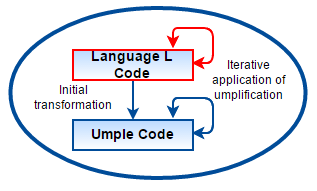
\includegraphics[width=0.50\textwidth]{Figures/UmplificationProcess.png}
\caption{The Umplification process generalized}
\label{fig:umplificationLoop}
\end{figure}

The umplification process has several properties. It is:
\begin{enumerate}
 \item \textbf{incremental}, 
 \item \textbf{transformational},
 \item \textbf{interactive},  
 \item \textbf{extensible}, and
 \item \textbf{implicit-knowledge} conserving. 
\end{enumerate}

The approach is \textbf{incremental} because it can be performed in multiple small steps that produce (quickly) a new version of the system with a small amount of additional modeling information, such as the presence of one new type of UML construct. At each step, the system remains compilable. The approach proceeds incrementally performing additional transformations until the desired level of abstraction is achieved.	These incremental transformations allow for user interaction to provide needed information that may be missing or hard to automatically obtain because the input (the source code) does not follow any of the idioms the automatic umplification tool is yet able to recognize. This characteristic of umplification allows developers, if they wish, to repeatedly re-introspect the transformed program and manually validate each change with an understanding of the incremental purpose of the change.

The approach is \textbf{transformational} because it modifies the original source rather than generating something completely new. It first translates the original language (Java, C++ etc.) to an initial Umple version that looks very much like the original, and then translates step-by-step as more and more modeling constructs are added, replacing original code.

The approach is \textbf{transformational} because the user's feedback may be used to enhance the transformations.

The approach is \textbf{interactive} because it uses the set of transformation rules can be readily extended to refine the transformation mechanism. 

Finally the approach is \textbf{implicit-knowledge} conserving because it preserves code comments, and, where possible, the layout of whatever code is not (yet) umplified. The latter includes as the bodies of algorithmic methods – known as action code in UML.

Taken together, the above properties allow developers to confidently umplify their systems without worrying about losing their mental model of the source code. Developers gain by having systems with a smaller body of source code that are intrinsically self-documented in UML. 

The following gives a summary of the abstract transformations currently implemented.
\begin{description} 
\item[Transformation 0: Initial transformation] 
To start, source files with language L (e.g. Java, C++) code are initially renamed as Umple files, with extension .ump. File, package and data type's inclusions are translated into Umple dependencies by using the depend construct. 
\item [Transformation 1: Transformation of generalization/specialization, dependency, and namespace declarations]
The notation in the base language code for subclassing is transformed into the Umple 'isA' notation. Umple now recognizes the class hierarchy.  Notations representing dependency are transformed into Umple 'depends' clauses, and notations for namespaces or packages are transformed into the Umple 'namespace' directives. At this stage, an Umple program, when compiled should generate essentially identical code to the original program.
\item [Transformation 2: Analysis and conversion of many instance variables, along with the methods that use the variables]
This transformation step is further decomposed into sub-steps depending on the abstract use of the variables. The sub-steps are defined as follows.
   \begin{description}
\item [Transformation 2a: Transformation of variables to UML/Umple attributes]
If variable a is declared in class A and the type of a is one of the primitive types in the base language, then a is transformed into an Umple attribute. Any accessor (e.g. getA()) and mutator (e.g. setA(…)) methods of variable a are transformed as needed to maintain a functioning system. In particular, any getter and setter methods in the original system must be adapted to conform to or call the Umple-generated equivalents.
\item [Transformation 2b: Transformation of variables in one or more classes to UML/Umple associations]
If variable a is declared in Class A and the type of a is a reference type B, then a is trans-formed into an Umple Association with ends {a, b}. At the same time, if a variable b in class B is detected that represents the inverse relationship then the association becomes bidirec-tional. The accessor and mutator methods of variable a (and b) are adapted to conform to the Umple-generated methods. Multiplicities and role names are recovered by inspecting both types A and B; this is explained in Section 3.3. 
\item [Transformation 2c: Transformation of variables to UML/Umple state machines]
If a is declared in Class A, has not been classified previously as an attribute or association, has a fixed set of values, and changes in the values are triggered by events, and not by a set method, then a is transformed to a state machine.	We will not cover this aspect of umplification further in this thesis, and will leave the focus on attributes and associations.
% If time allows, state machines will be cover since I have some rules for it. 
As mentioned before, as part of each transformation step, the accessor, mutator, iterator and event methods are adapted (refactored) to conform to the Umple generated methods. Table \ref{table:transformations} summarizes these additional required refactorings. 
   \end{description}

\end{description}

\begin{table}[htbp]
	\caption{Refactorings to methods required for each transformation}
	\label{table:transformations}
    \centering
    \begin{tabularx}{\textwidth}{| X | X |}
    %\begin{tabularx}{\textwidth}{sb}
        \toprule
        \rowcolor[HTML]{BBDAFF}
       \textbf{ Transformation case  }   & \textbf{Method Transformations}
        \\ \hline
        \textbf{(0)  Classes }        & None      \\ \hline
        \textbf{(1)  Inheritance}     & None       \\ \hline
        \textbf{2a)  Attributes}      & 
        Accessor (getter) and mutator (setter) methods are removed from the original code 				if they are simple since Umple-generated code replaces them. Custom accessors and 				mutators are refactored so Umple generates code that maintains the original
        semantics.         		\\ \hline
        \textbf{(2b) Associations }   & 
 		Accessor and mutator methods are removed or correctly injected into the umple code.        
		\\ \hline
        \textbf{(2c) State Machines  }  & 
		Methods triggering state change are removed if they are simple (just change state) or 		modified to call Umple-generated event methods. Not covered further in this 					paper       		
\\ \hline
    \end{tabularx}
\end{table}

In the following chapter, we provide a more detailed view of the transformation cases. To help distinguish between Umple and Java code presented in this thesis, the Umple examples appear in solid borders with blue shading, pure Java examples have solid borders with green shading. Mapping rules (in the Drool language, that we will describe in Chapter 5) appear using single line borders with no shading. 